\chapter{Tecnologías}
\label{cap:introduccion}

%\chapterquote{}{}

\begin{resumen}
	En este capítulo se enumerarán las tecnologías utilizadas y su utilidad en el proyecto.
\end{resumen}

\label{cap1:sec:Motivacion}


\section{Introducción}

La finalidad de PictUp! es crear una aplicación web accesible desde el ordenador que permita crear materiales pictográficos. La aplicación se ha desarrollado en React y para facilitar la maquetación de la misma se ha utilizado Boostrap 5\footnote{\url{https://getbootstrap.com/docs/5.0/getting-started/introduction/}}. 
A continuación se describirán estas y otras tecnologías estudiadas de cara al desarrollo de PictUp!.


\section{API Arasaac}
\label{cap3:sec:apiarasaac}
ARASAAC facilita la obtención de recursos pictográficos mediante su API\footnote{\url{https://arasaac.org/developers/api}}. Una API es una interfaz que reúne un conjunto de funciones y métodos, accesibles para otras aplicaciones. En el caso de la API de ARASAAC, esta está exclusivamente disponible para aplicaciones no comerciales, tal y como indica su licencia Creative Commons.
Mediante los métodos de la API , podemos obtener materiales y pictogramas. Los materiales  son actividades, calendarios o agendas creados por usuarios haciendo uso de los pictogramas de ARASAAC. Respecto a los pictogramas, los métodos que se han utilizado en este trabajo son:

\begin{itemize}
	\item \textbf{bestSearch}: recibe una palabra y retorna un único JSON con la información del pictograma que más se ajuste a la palabra.
	
	\item \textbf{searchText}: igual que \textit{bestSearch}, diferenciándose en que retorna todos los pictogramas similares. En la Figura \ref{fig:compBusq}, se ejemplifica el resultado de introducir el mismo término en las dos funciones.
	
	 \begin{figure}[h!]
	 	\centering
	 	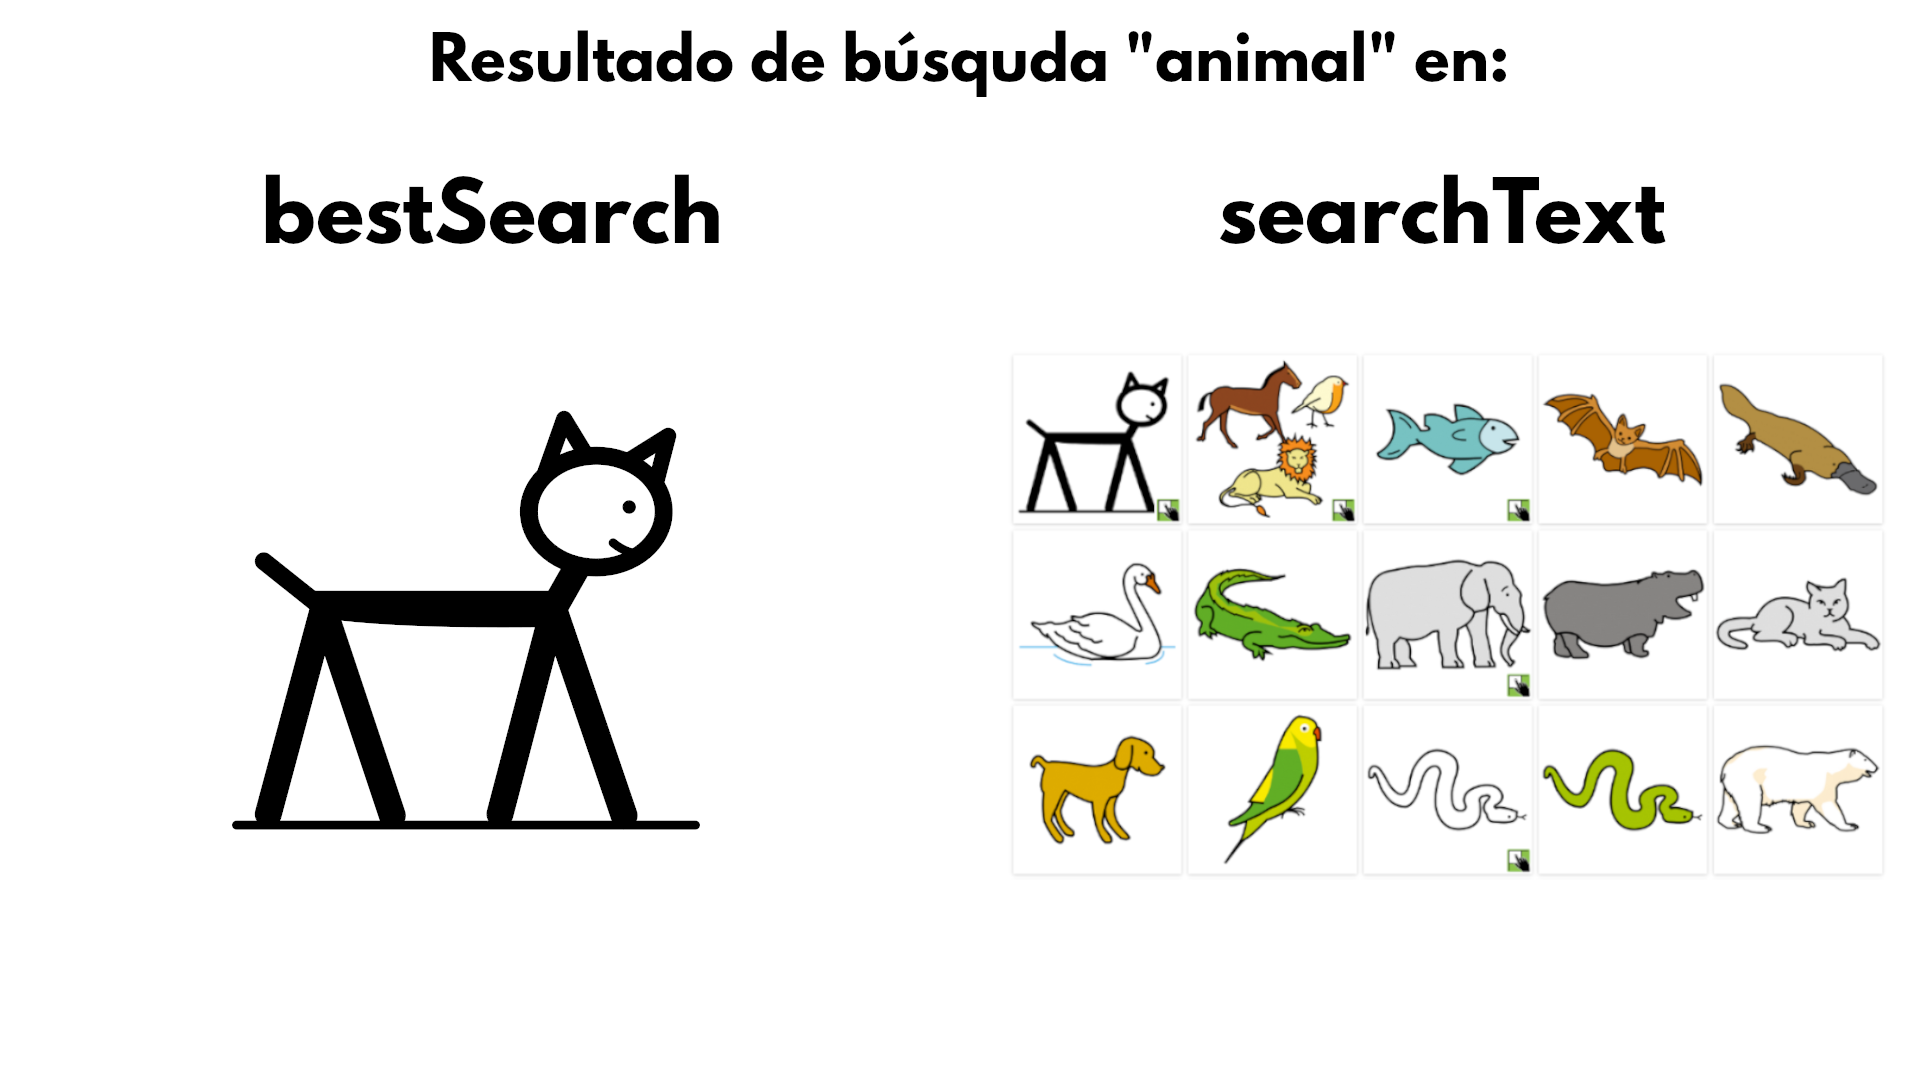
\includegraphics[width=0.8\linewidth]{Imagenes/Bitmap/techComparacionBusquedas}
	 	\caption{Comparación de los resultados con ambas búsquedas}
	 	\label{fig:compBusq}
	 \end{figure}
	
	\item \textbf{idPictogram}: a partir del identificador de un pictograma, retorna la dirección de la imagen del pictograma asociado al identificador.    
\end{itemize}


Como se ha mencionado anteriormente, la API de ARASAAC retorna un objeto JSON que almacena toda la información de un pictograma. Los parámetros más importantes que tiene un objeto pictograma son: 



\begin{itemize}
	\item \textbf{\_id}: número único que lo identifica, se utiliza para cargar la imagen.
	
	\item \textbf{keyword}: la palabra asociada al pictograma.
	
	\item \textbf{hasLocution}: indica si cuenta con locución. La locución está grabada por una persona y no se trata de una voz robótica generada automáticamente.
	
	\item \textbf{hair}: indica si el pictograma representado tiene pelo. En caso afirmativo, se podrá cambiar el color de éste.
	
	\item \textbf{skin}: indica si el pictograma representa a una persona. En caso afirmativo, se podrá cambiar el tono de piel. 
	
\end{itemize}

Los pictogramas pueden ser personalizados, como se puede ver en la Figura \ref{fig:colorespicto}. La web cuenta con un mayor rango de opciones, como tachar un pictograma, añadir un marco o cambiar el color de fondo. Aunque la API es más limitada y cuenta con menos opciones, éstas son: cambiar el color de pelo y piel si el pictograma  lo permite, indicar plural, tiempo verbal y dejarlo en blanco y nego. Esta personalización no se obtiene directamente desde la API, sino que se ha de modificar una URL en función de los atributos modificados para que el pictograma aparezca de manera diferente. 

\begin{figure}[h!]
	\centering
	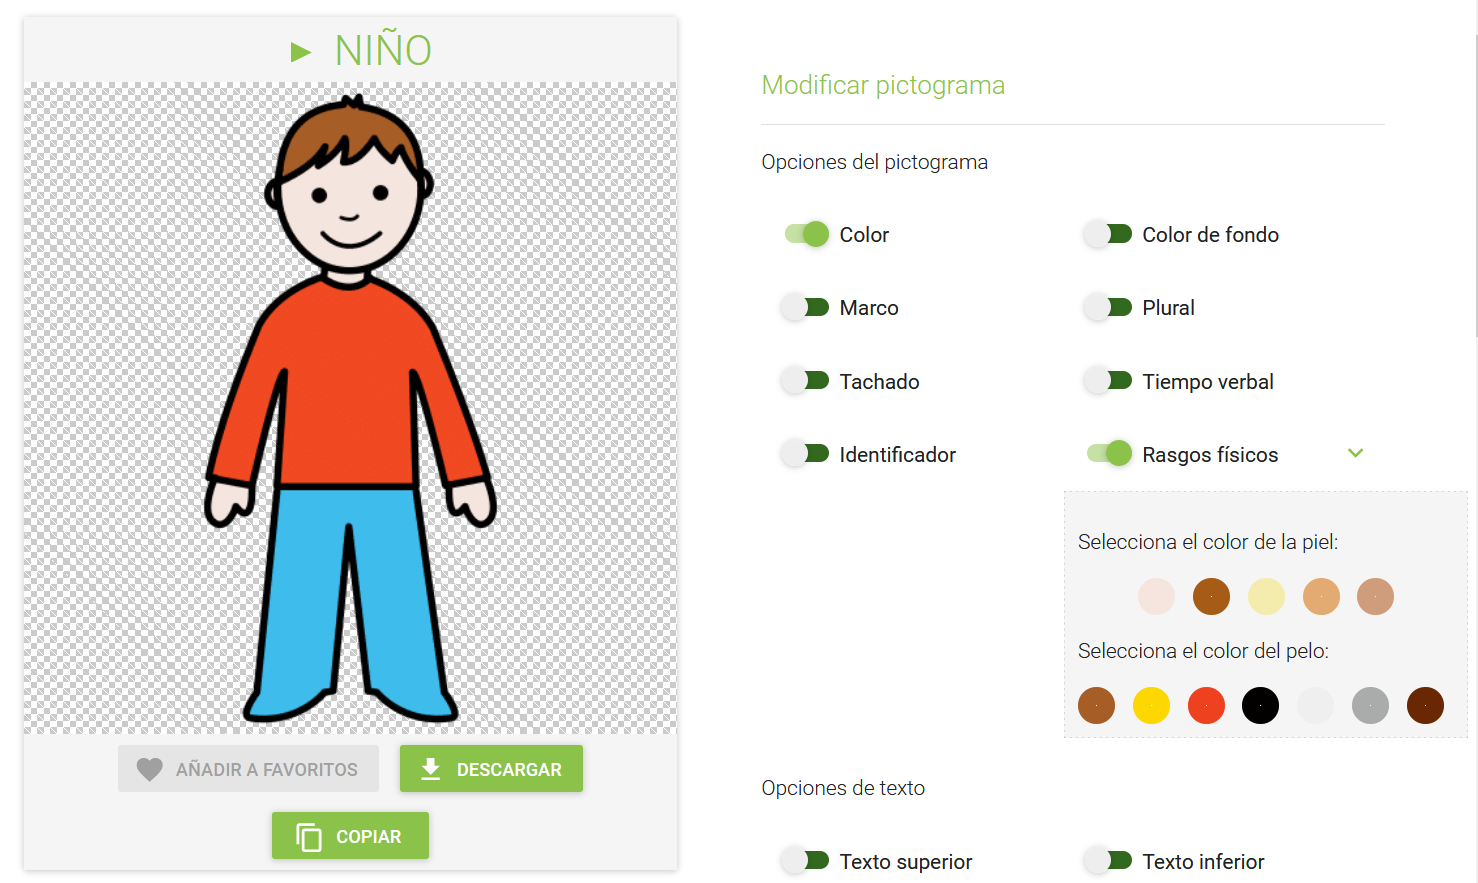
\includegraphics[width=0.7\linewidth]{Imagenes/Bitmap/coloresPicto}
	\caption{Ejemplo de cómo se puede modificar el color de pelo y tono de piel de un pictograma, entre otras opciones, en este caso desde la web de ARASAAC.}
	\label{fig:colorespicto}
\end{figure}
\subsection{Prototipo API ARASAAC}
Para probar el acceso a la API se creó un sencillo buscador de pictogramas utilizando el método \textit{bestSearch} para comprender el funcionamiento de la API y las posibilidades que ésta ofrece. Aunque inicialmente simplemente muestra el pictograma de una palabra introducida, durante el desarrollo añadimos la posibilidad de cambiar el color de pelo, tono de piel y otros atributos de los pictogramas.

\section{React}
\label{cap3:sec:react}
React es una librería de Javascript pensada para desarrollar interfaces de usuario. Esta librería fue desarrollada por Facebook buscando la creación de interfaces de una manera sencilla y con un alto rendimiento. 
React permite desarrollar tanto aplicaciones web como aplicaciones móviles de una manera ordenada y con menos líneas de código respecto a otros lenguajes como Javascript. El hecho de que React permita estructurar los distintos componentes de una aplicación ayuda tanto al desarrollo como mantenimiento de esta.
Otra característica importante de React es que ya tiene implementadas muchas funcionalidades, por lo que puede ayudar a reducir el tiempo de desarrollo de la aplicación. Un ejemplo de esto es el hecho de tener las vistas asociadas a los datos, que permite que los datos mostrados se actualicen automáticamente sin necesidad de escribir nuevos fragmentos de código.

Respecto a otros Frameworks como Angular, vemos que React no ofrece todas las funcionalidades de un framework completo. Esto no supone ningún impedimento para desarrollar la aplicación con React pero habrá que adaptar nuestro código al ecosistema que ofrece.



\subsection{Drag and Drop}
\label{cap3:sec:draganddrop}
React Drag and Drop\footnote{\url{https://react-dnd.github.io/react-dnd/about}} es una biblioteca que permite arrastrar componentes en React. Su principal uso en la aplicación es la recolocación de los componentes del tablero de manera cuadriculada. Esto permite colocar con precisión los elementos en el tablero, lo cual era un requisito indispensable para poder hacer tableros organizados. De otra manera podrían quedar algunos componentes unos pocos píxeles por encima de otros, dando un resultado sin alinear y poco profesional.

\subsection{Prototipos}
\label{cap3:sec:prototipos}
Otro objetivo es el de la interacción de los componentes en una superficie cuadriculada. Tras experimentar con distintas bibliotecas de JavaScript como Interact JS \footnote{\url{https://interactjs.io/}} no obtuvimos el resultado esperado pues el desplazamiento de los objetos no era lo suficientemente preciso.

React tenía la biblioteca Drag and Drop que permite desplazar los componentes. La principal diferencia entre Drag and Drop y Interact JS, es que al mover un elemento, “Interact JS”  deja unos píxeles de diferencia y “Drag and Drop.” permite mover objetos en intervalos definidos, como poder mover un objeto de 10 píxeles en 10 píxeles.

\section{JSZip}
\label{cap3:sec:jszip}
JSZip\footnote{\url{https://stuk.github.io/jszip/}} es una biblioteca de Javascript que mediante una API permite crear y cargar archivos comprimidos en formato \textit{ZIP}. Será el método para importar y exportar elementos de la aplicación.
\begin{itemize}
	\item \textbf{Generar ZIP}: Crea un zip con todo lo que haya creado el usuario, como las fotos que haya subido, la posición de los pictogramas colocados y su información asociada.
	\item \textbf{Cargar ZIP}: Al subir un ZIP, descomprime su contenido para poder cargar los elementos en la aplicación.
\end{itemize}	


\section{Progressive Web Application}
\label{cap3:sec:pwa}

Las aplicaciones web progresivas (PWA)\footnote{\url{https://developer.mozilla.org/en-US/docs/Web/Progressive_web_apps}} son aplicaciones instalables en ordenador o dispositivos Android. Están a medio camino entre una aplicación nativa\footnote{\url{https://web.dev/what-are-pwas/}}  y una web, pues ofrecen más posibilidades que una web convencional y no requiere de instaladores o ser descargadas de tiendas de aplicaciones.
    
Entre otras ventajas que se ofrecen:

\begin{itemize}
	\item Los tiempos de carga son reducidos al contar con los componentes precargados.
	
	
	\item Son fáciles de instalar.
	
	\item Añade un icono a la pantalla de inicio del móvil o un acceso directo en el escritorio donde se instala, aumentando las posibilidades que el usuario vuelva a acceder a la aplicación. Debido a que una web puede ser muy difícil de encontrar en motores de búsqueda, el usuario puede ser dependiente de tener el enlace a su alcance.
	
	\item Ahorra el desarrollo de una aplicación nativa para Android. 
	
	\item Son rápidas y fáciles de implementar.
	
\end{itemize}

Actualmente las PWA son accesibles desde la gran mayoría de navegadores tanto de ordenador como móvil.






